%% from aastex61.cls with a few tweaks to allow for the unique format required.
\documentclass{rnaastex}

\begin{document}

\title{Spectral-line broadening from finite channel widths}

%% Note that the corresponding author command and emails has to come
%% before everything else. Also place all the emails in the \email
%% command instead of using multiple \email calls.
COrrespondingauthor{Eric Koch}
\email{ekoch@ualberta.ca}
\author[0000-0001-9605-780X]{Eric Koch}
\author[0000-0002-5204-2259]{Erik Rosolowsky}
\affiliation{University of Alberta, Department of Physics 4-183 CCIS, Edmonton AB T6G 2E1, Canada}


%% Note that RNAAS manuscripts DO NOT have abstracts.
%% See the online documentation for the full list of available subject
%% keywords and the rules for their use.
\keywords{}

%% Start the main body of the article. If no sections in the
%% research note leave the \section call blank to make the title.

\section{}

When the number of channels across the FWHM of a Gaussian profile decreases, the sampling of the line profile becomes important for determining the spectral properties.  This is most often addressed in the literature for the line width, where a correction factor is often applied to remove the effect of broadening due to the spectral channels \citep[e.g.,][]{cprops2006PASP..118..590R}. This correction factor is often taken to be the effective Gaussian width from setting the area in one spectral channel equal to the integral of a Gaussian:
\begin{equation}
    \label{eq:width_corr_fact}
    \sigma_{\rm response} \approx \frac{\Delta v_{\rm channel}}{\sqrt{2\pi}}.
\end{equation}
Other authors have adopted larger correction factors XXX that GBT paper w/o the sqrt on the bottom XXX.

Sampled with finite channels, a Gaussian profile will be measured as the average value of the Gaussian within the channel limits.  For channel centered at $v$ with width $\Delta v$, the measured value of a Gaussian centered at $\mu$ with a peak of $A$ and width of $\sigma$ will be
\begin{equation}
    \label{eq:finite_gaussian}
    G(v) = \frac{A}{(\Delta v)^2} \left[ {\rm erf}\left( \frac{\mu - (v - \Delta v / 2)}{\sqrt{2}\sigma} \right) - {\rm erf}\left( \frac{\mu - (v + \Delta v / 2)}{\sqrt{2}\sigma} \right) \right].
\end{equation}
Figure \ref{fig:gaussian_finite_model} shows the discrepancy between the true Gaussian model and the model produced with Equation \ref{eq:finite_gaussian}. As the ratio of $\sigma / \Delta v$ decreases, the discrepancy between the Gaussian profile and the finitely-sampled version increase, where $\sigma$ is overestimated and $A$ is underestimated. Figure \ref{fig:gaussian_finite_model} also shows the discrepancy between sampling the Gaussian model at only the channel centre versus accounting for the whole channel width.


There is additional line broadening from the response function of the spectrometer.  The previous example is the case of a perfect spectral response, where each channel is independent of the others.  Real spectrometers have a response function that correlates nearby channels.  It is also common to Hanning smooth data, which, without spectral downsampling, will also yield correlated spectral channels.  For some instruments, the response function is well-characterized and can be directly included in the model for a spectral line XXX Rosolowsky NH3 GBT, recent sitelle fitting papers XXX.  In the absence of an analytic expression for the response function, the typical channel-to-channel correlation can be used to approximate the response function. \citet{Leroy2016ApJ...831...16L} characterize the typical XXX

\citet{Leroy2016ApJ...831...16L} and \citet{Sun2018ApJ...860..172S} find that the IRAM-30m CO(2-1) data used here are correlated with the nearest channels; \citet{Sun2018ApJ...860..172S} find a channel-to-channel correlation of $r=0.26$ for the IRAM-30m CO(2-1) data.  These studies use a version of the data that has additional noise added to remove spatial variations in the noise.  However, we find no significant difference in the channel correlations and adopt the value from \citet{Sun2018ApJ...860..172S}. XXX Hanning kernel XXX

XXX Compare different line width estimators at different sigma to channel width ratios, and with/without broadening and the ad hoc channel correction XXX
We compare these different estimates of the line width as a function of $\sigma/\Delta v$ in Figure XXX. XXX

\begin{figure*}
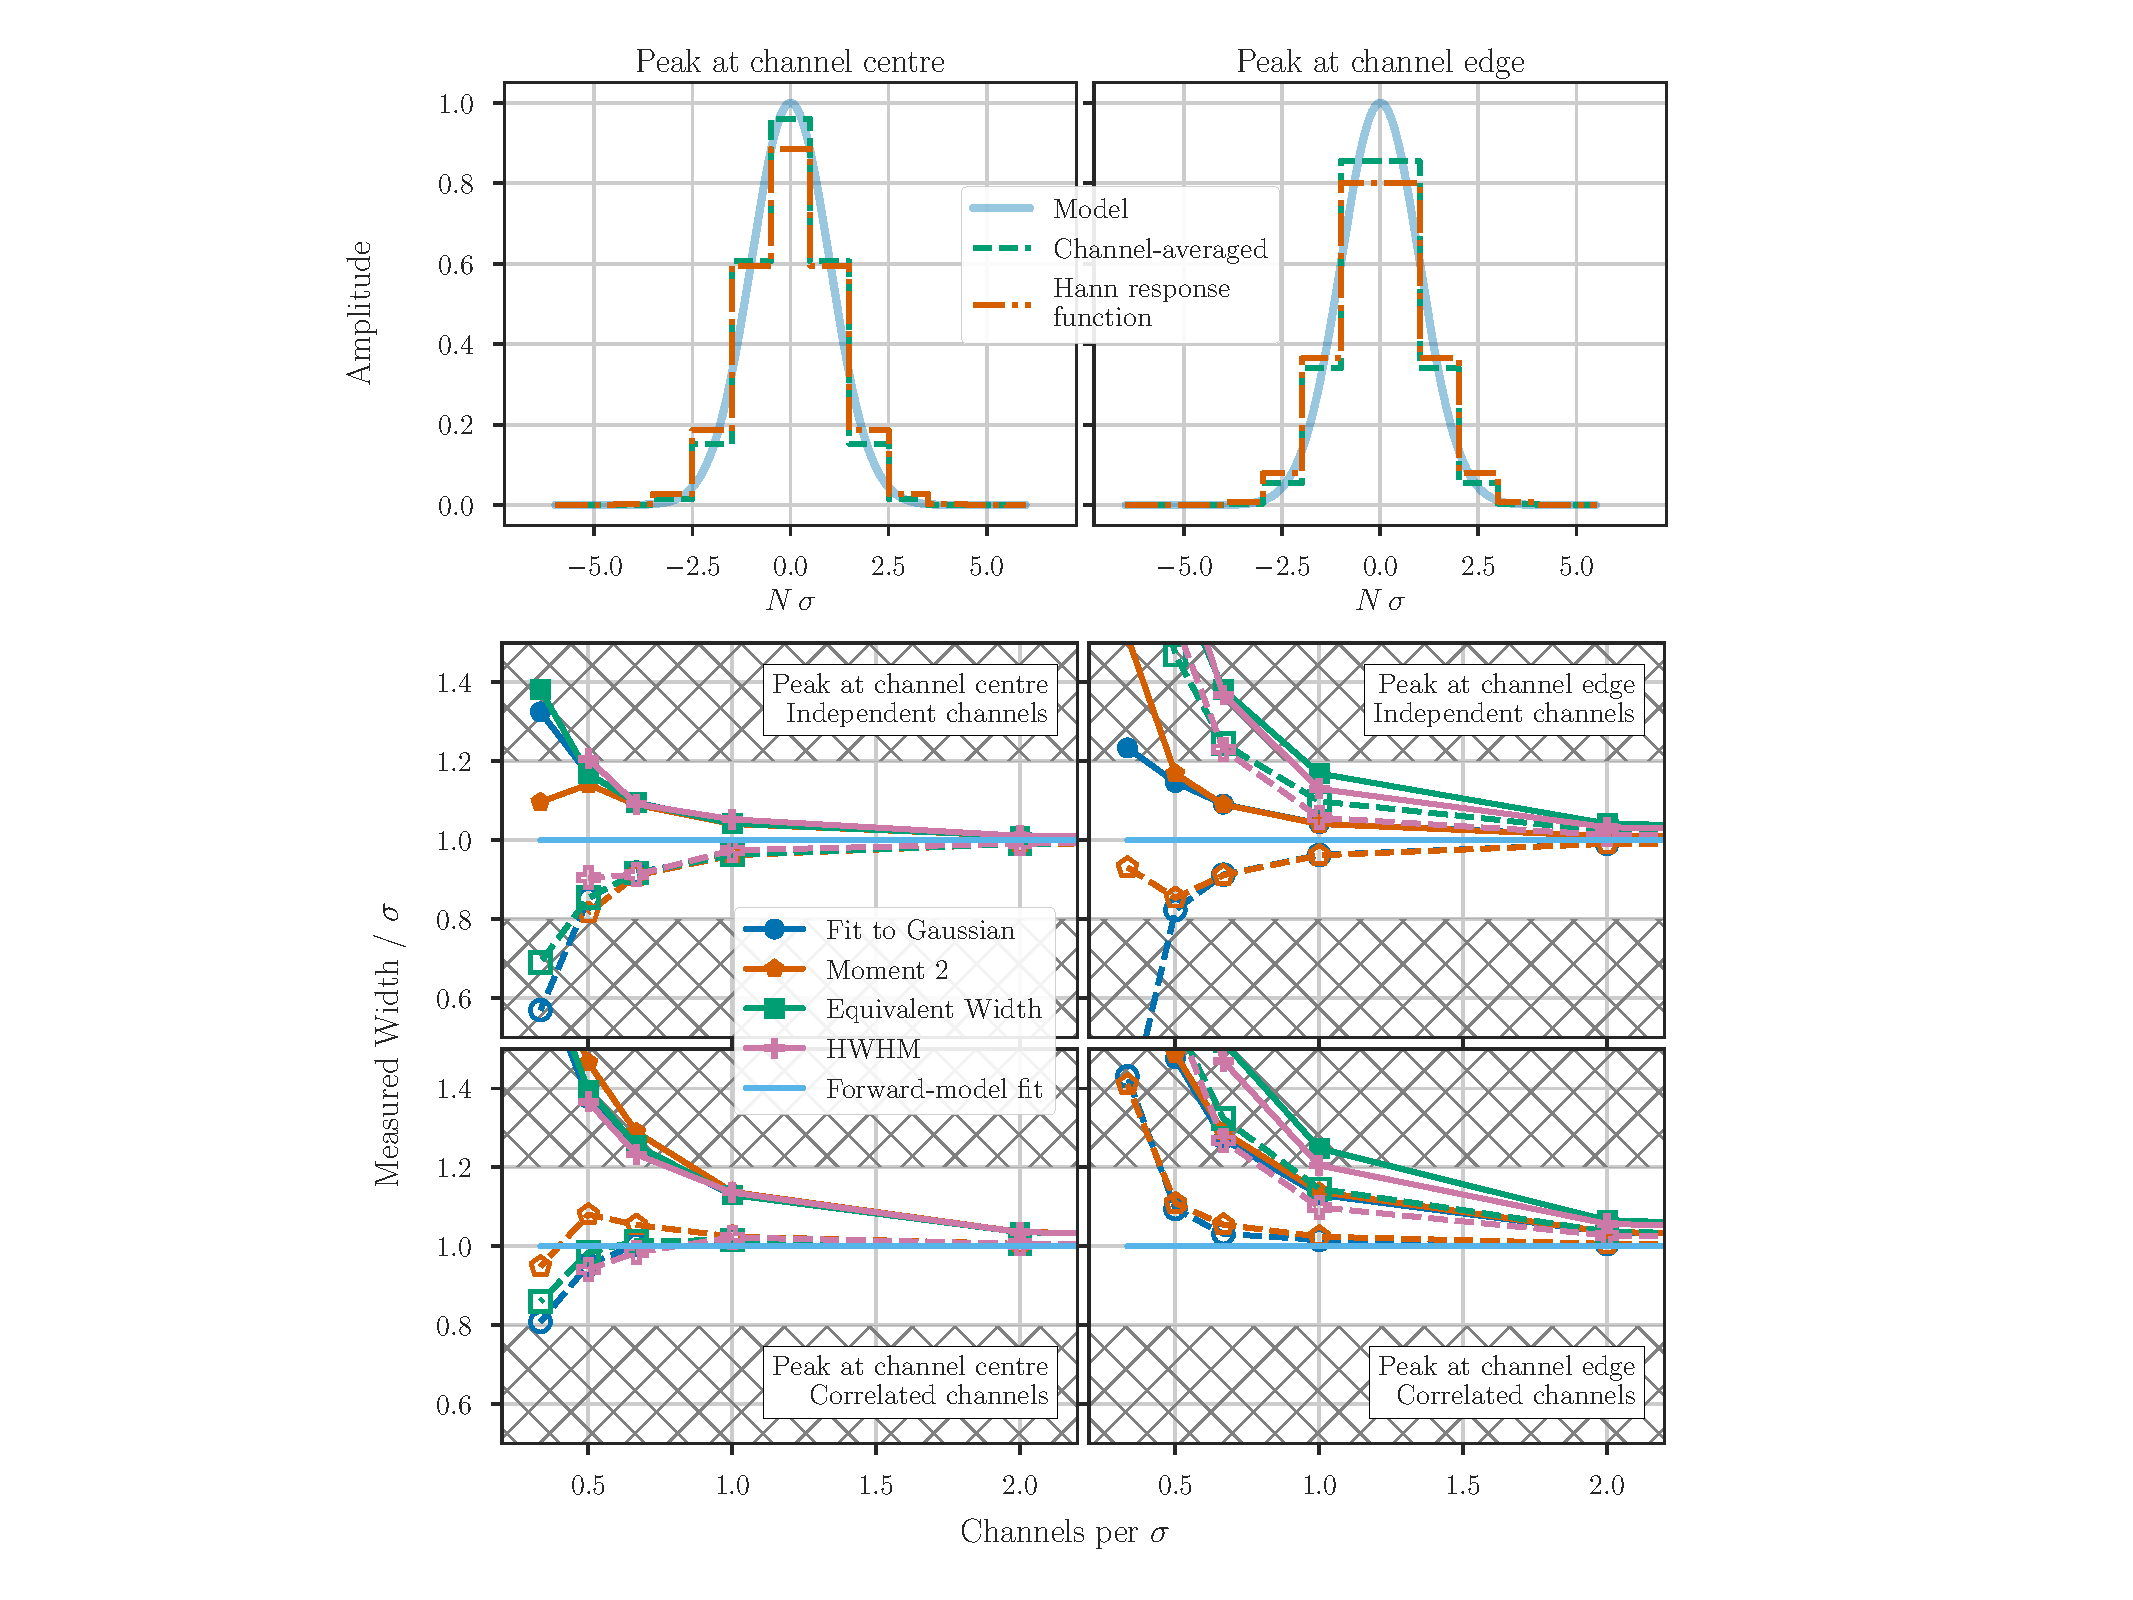
\includegraphics[width=\textwidth]{combined_figure}
\caption{\label{fig:width_recovery_comparison} Comparison of methods for recovering the width of a noiseless Gaussian model as a function of the number of channels per $\sigma$. The first row of panels are width estimates for a Gaussian sampled with Equation \ref{eq:finite_gaussian}, while the second row panels are also convolved by a Hanning kernel of $[0.XXX,, 0.XXX]$ to mimic a realistic spectral response.  The first column shows width estimates when the ture model peak is located at the channel centre (best-case) and the second column are widths when the peak is located at the channel edge (worst case).  The solid lines are the width estimates and the dashed lines are the widths after deconvolving with the empirical relation from \citet{Leroy2016ApJ...831...16L}.}
\end{figure*}

Since the correction factor that has previously been adapted for the effect of broadening over-corrects the line width, we choose to directly include the finite channel sampling and smoothing from an approximate Hanning kernel into the model.  This is a simple example of ``forward modelling'' to account for known systematic effects.  Figure XXX shows that fitting with these effects correctly recovers the line width and amplitude to $\sigma/\Delta v = XXX$.  We use this approach for fitting the CO spectra in \S\ref{sub:hi_line_widths_associated_with_co}.  Since the {\sc HI} spectral resolution is significantly higher, and the {\sc HI} line widths tend to be larger than the CO, the {\sc HI} spectra will not be significantly broadened from these effects and we do not account for them when fitting the {\sc HI} spectra.

The examples above do not include noise in the spectra. We fit the spectral Gaussian model, including broadening from a Hanning kernel, to 1000 spectra with Gaussian noise added.  The noise is added prior to the convolution to produce realistic spectra, and the standard deviation of the noise distribution is set to give a peak S/N of $3$ in the spectra.  The distributions of fitted parameters are centered at the correct values, confirming that the model is not biased.

The spectra are fit with the Levenberg-Marquadt algorithm.  We note that this algorithm treats the uncertainty in each spectral channel as independent, which is not correct due to the spectral response function.  To determine whether this biases the parameter uncertainties, we calculate a p-value from the 1000 iterations testing the number of times the true parameter value falls within the fitted $1\mbox{-}\sigma$ uncertainty range.  The mean velocity, standard deviation, and amplitude of the Gaussians each have p-values within $0.02$ of $0.68$, as expected for a two-tailed p-value within $1\mbox{-}\sigma$.  Thus we do not attempt to model correlated uncertainties for the CO(2-1) LOS fitting in \S\ref{sub:hi_line_widths_associated_with_co}. If spectral channels are highly correlated, or are correlated beyond their nearest neighbors, a Gaussian Process could be used to account for correlations in the model XXX rasmussen and williams XXX.

Comparing different commonly-used line width estimates, we find that each method is biased to larger values as the channel width approaches the width of the spectral line.  The often-assumed correction factor for this line width broadening does not consistently work in any case.  The line width broadening is a strong function of where the peak position is located with respect to the channel centre.  Because of this dependence, there is no single correction factor that can account for the line width broadening.  When simulating the additional broadening due to a spectral response function, we find that the empirically-derived correction formula from \citet{leroy16}, which depends on the channel-to-channel noise correlation, correctly account for line width broadening if the peak of the spectral-line is near the channel centre.

Correctly accounting for line width broadening requires forward modelling for the finite channel width and the spectral response function.  We present a forward modelling analysis for the simplest case, a single Gaussian profile, and demonstrate that it can correctly recover line properties for unresolved spectra in the noiseless case.  With added noise, a spectrum must be at least Nyuquist-sampled to recover meaningful line properties.  We show that forward modelling correctly recovers the line width parameters to within the uncertainty for spectra that are sampled with channels equal to $\sigma$ with a peak signal-to-noise of $3$.

The forward-modelling shown here can be extended to arbitrary spectral line models by numerically calculating the model within each spectral bin when an analytic expression does not exist XXX.

%% An example figure call using \includegraphics
% \begin{figure}[htp!]
% \begin{center}
% \includegraphics[scale=0.65,angle=0]{oh_figure.pdf}
% \caption{\label{fig:1} Right: Position of the OH detection on an integrated 21-cm map of M33 (Koch et al., in prep). Top Left: Spectrum at the peak intensity position. The dashed green line is the noise level at 1.85 mJy and the thick orange line is a Gaussian fit. Bottom Left: H$\alpha$ image of the region shown in the right panel \citep{hodge1999}.  Sources from the \citet{moody2017} catalogue are shown in blue within the beam area, and green for nearby regions [from left to right, C1-10 \citep{moody2017}, 79a and 79c \citep{boul1974}].}
% \end{center}
% \end{figure}

\acknowledgments

EWK is supported by a Postgraduate Scholarship from the Natural Sciences and Engineering Research Council of Canada (NSERC). EWR acknowledges the support of NSERC, funding reference number RGPIN-2017-03987.

\software{}

\begin{thebibliography}{}

\end{thebibliography}

\end{document}
